\begin{graphicspathcontext}{{./chapters/its/imgs/},{./chapters/its/imgs/auto/},\old}

\section{General Context}

\begin{textpictureframe}{Digital Transformation}{digital-transformation}
	\begin{itemize}
	\item Worldwide data volume doubles every two years. By 2020, it will have grown to 40 zettabytes --- a 50-fold increase within 10 years
	\item Worldwide revenue of the IT and communications industries reached a record
\euro\ 2.84 trillion in 2013
	\item Revenue from apps alone amounted to \euro\ 66.2 billion in 2013 and has more than
double in 2017
	\item Digitalization boosts GDP --- a 10\% increase in the digitalization level of a country leads to 0.75\% rise in per capita GDP
	\end{itemize}
\end{textpictureframe}

\begin{textpictureframe}{Urbanization}{urbanization}
	\begin{block}{Growth of cities}
	\begin{description}
	\item[2009] For the first time in history, more than 50\% of the world's population lived in cities
	\item[2050] 70\% of the world's population will live in cities
	\end{description}
	\end{block}
	\begin{block}{Megacities worldwide}
	\begin{description}
	\item[1970] 2 megacities with more than 10 million inhabitants
	\item[2025] 37 megacities; more than 13\% of the world's population will live in a megacity
	\end{description}
	\end{block}
\end{textpictureframe}

\begin{textpictureframe}{Demographic Change}{demographic-change}
	\begin{block}{World population}
	\begin{description}
	\item[2012] 7.1 billion people
	\item[2050] 9.6 billion people
	\end{description}
	\end{block}
	\begin{block}{Worldwide life expectancy}
	\begin{description}
	\item[2012] 70 years
	\item[2050] 76 years
	\item By \alert{2050}, the share of the population aged 60 or over will, for the first time, equal the share of the population younger than 15
	\end{description}
	\end{block}
\end{textpictureframe}

\begin{textpictureframe}{Climate Change}{climate-change}
	\begin{description}
	\item[2012] \\
		Highest CO\textsubscript{2} concentration in the atmosphere in 800,000 years
	\item[2001 to 2010] \\
		Warmest decade on record
	\end{description}
\end{textpictureframe}

\figureslide[width=.8\linewidth]{{Need Radical Changes} in Transport Systems}{systems_simple}

\section[Definition]{Definition of Intelligent Transport Systems}
 
\begin{frame}{What is an Intelligent Transport Systems?}
	\begin{definitionblock}{Intelligent Transport Systems (ITS)}
		Systems in which information and communications technologies are applied to transport infrastructure and vehicles
	\end{definitionblock}
	\vspace{1em}
	\begin{block}{ITS improves}
		\begin{itemize}
		\item Transport safety
		\item Transport productivity
		\item Travel reliability
		\item Informed travel choices
		\item Social equity
		\item Environmental performance
		\item Network operation resilience
		\end{itemize}
	\end{block}
\end{frame}

\section[Technologies]{Technologies related to ITS}

%\animatedfigureslide<1-2>{Intelligent Transport Technologies}{itt}
\figureslide[width=.8\linewidth]{Intelligent Transport Technologies}{itt_simple1}

\begin{frame}{Wireless Communication}
	\begin{columns}
		\begin{column}{.4\linewidth}
			\small
			\begin{itemize}
			\item Radio communication (\emph{UHF}, \emph{VHF} frequencies) for short/long range communication
			\vspace{1em}
			\item \emph{IEEE 802.11 protocols} for short-range communications (less than 450 meters)
			\vspace{1em}
			\item \emph{WiMAX (IEEE 802.16), Global System for Mobile Communications (GSM), or 3G/4G} for longer range communications
			\end{itemize}
		\end{column}
		\begin{column}{.6\linewidth}
			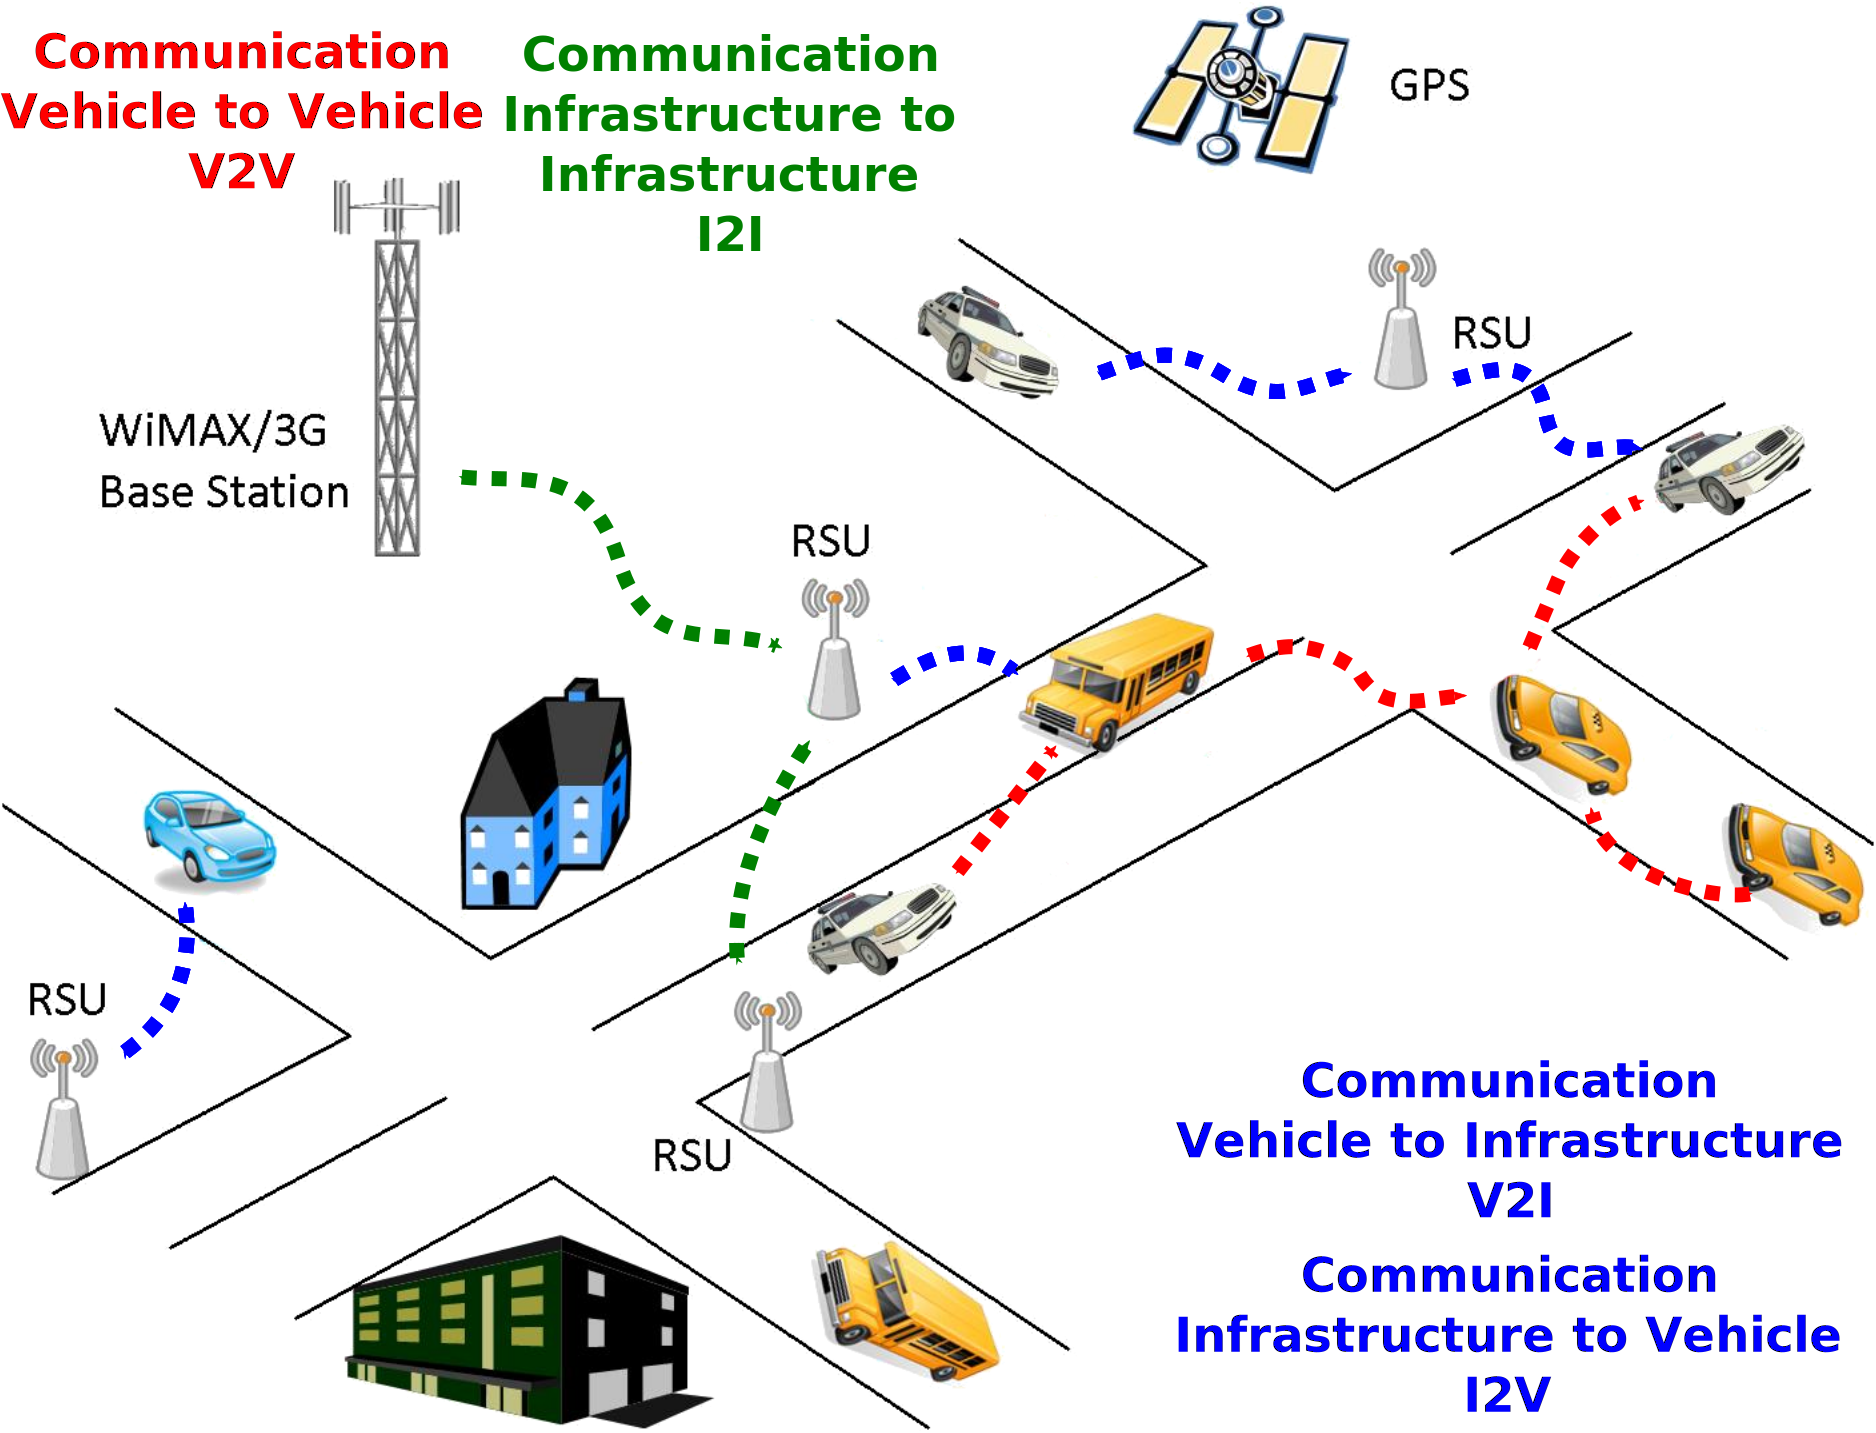
\includegraphics[width=\linewidth]{wireless_simple}
		\end{column}
	\end{columns}
\end{frame}

%%\animatedfigureslide{Example: Join a road train}{joinaroadtrain}
%\figureslide{Example: Join a road train}{joinaroadtrain_simple1}
%\figureslide{Example: Join a road train}{joinaroadtrain_simple2}
%\figureslide{Example: Join a road train}{joinaroadtrain_simple3}
%\figureslide{Example: Join a road train}{joinaroadtrain_simple4}
%\figureslide{Example: Join a road train}{joinaroadtrain_simple5}
%\figureslide{Example: Join a road train}{joinaroadtrain_simple6}
%\figureslide{Example: Join a road train}{joinaroadtrain_simple7}

%\animatedfigureslide<4>{{Floating Car} / Cellular Data}{itt}
\begin{frame}{{Floating Car} and Cellular Data}
	\begin{description}
	\item[Provides]
		\begin{itemize}
		\item travel speed 
		\item time data...
		\end{itemize}
	\item[Advantages]
		\begin{itemize}
		\item Less expensive than sensors or cameras
		\item More coverage (potentially including all locations and streets)
		\item Faster to set up and less maintenance
		\item Works in all weather conditions, including heavy rain
		\end{itemize}
	\end{description}
	\vspace{1em}
	\begin{columns}
		\begin{column}{.5\linewidth}
			\alertbox*{Triangulation Method}
		\end{column}
		\begin{column}{.5\linewidth}
			\alertbox*{GPS}
		\end{column}
	\end{columns}
\end{frame}

\begin{frame}{Positioning: Triangulation Method}
	\begin{columns}
		\begin{column}{.7\linewidth}
			\begin{description}
			\item[Mobile phones as anonymous traffic probes]
				\begin{itemize}
				\item Mobile phones are moving with the vehicles
				\item Measuring and analyzing network data using triangulation, pattern matching or cell-sector statistics \\
				$\Rightarrow$ converted into traffic flow information
				\end{itemize}
			\vspace{.5cm}
			\item[Advantage] no infrastructure needs; only the mobile phone network
			\vspace{.5cm}
			\item[Trend] popularity is declining since 2010s
			\end{description}
		\end{column}
		\begin{column}{.3\linewidth}
			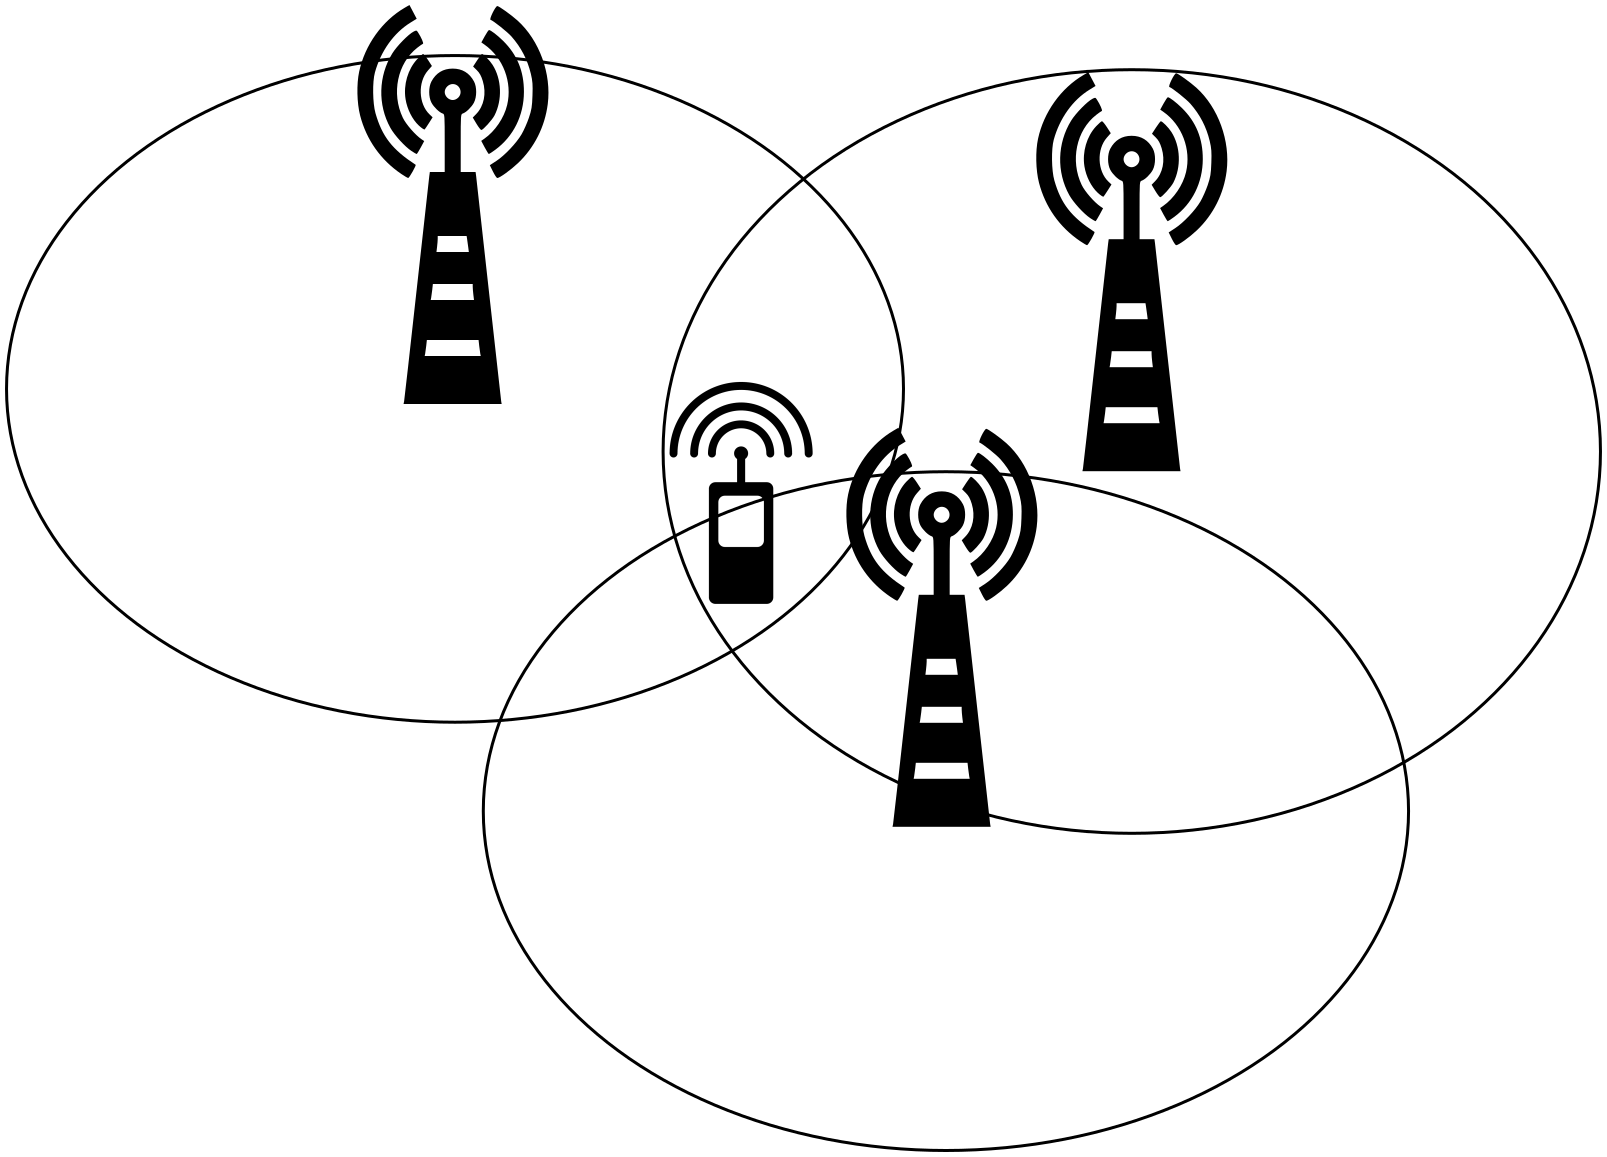
\includegraphics[width=\linewidth]{triangulationmethod}
		\end{column}
	\end{columns}
\end{frame}

%\animatedfigureslide<5>{Sensor Technologies}{itt}
\sidenote{Image generated by Claude Sonet 4.6}
\figureslide{Sensor Technologies}{its_sensors}

%\animatedfigureslide<6>{{Inductive Loop} Detection}{itt}
\begin{frame}{{Inductive Loop} Detection}
	\begin{columns}
		\begin{column}{.5\linewidth}
			\begin{itemize}
			\item Placed in a roadbed to detect vehicles
			\vspace{1em}
			\item Simplest detectors count the number of vehicles
			\vspace{1em}
			\item More sophisticated sensors estimate the speed, length, and weight of vehicles and the distance between them
			\end{itemize}
		\end{column}
		\begin{column}{.5\linewidth}
			\includegraphics[width=\linewidth]{its_inductiveloop}
		\end{column}
	\end{columns}
\end{frame}

%\animatedfigureslide<7>{Video Vehicle Detection}{itt}
\begin{frame}{{Video Vehicle} Detection}
	\begin{columns}
		\begin{column}{.4\linewidth}
			\begin{description}
			\item[Technologies] Video cameras (gray-scale, color, 2D, 3D)
			\vspace{.5cm}
			\item[Measurements] Traffic flow, incident detection using
			\vspace{.5cm}
			\item[Advantage] ``non-intrusive'' $\rightarrow$ no component directly into the road surface or roadbed
			\vspace{.5cm}
			\item[Constraint] Require machine learning or details on the camera configuration
			\end{description}
		\end{column}
		\begin{column}{.6\linewidth}
			\includegraphics[width=\linewidth]{its_videodetector1}
		\end{column}
	\end{columns}
\end{frame}

\section<3->[Applications]{Examples of Intelligent Transport Applications}

\subsection{Emergency vehicle notification systems}

\figureslide{eCall Alert System (H2020)}{ecall}

\begin{frame}[t]{Belfort-Montb\'eliard Highway Simulation}
\begin{center}
	\embeddedvideo[width=.78\linewidth]{./videos/its/aremis.avi}{screen2} \\
	Simulation of emergency situation on a french highway \cite{Buisson2014b}
\end{center}
\end{frame}

\subsection{Automatic road enforcement}

\begin{frame}{Automatic Road Enforcement}
	\begin{description}
		\item[Speed cameras] identify vehicles traveling over a legal speed limit (radar to detect vehicle's speed, electromagnetic loops buried in each lane)
		\vspace{.5cm}
		\item[Red light cameras] detect vehicles that cross while a red traffic light is showing
		\vspace{.5cm}
		\item[Bus lane cameras] identify vehicles traveling in lanes reserved for buses
		\vspace{.5cm}
		\item[Level crossing cameras] identify vehicles crossing railways at grade illegally
		\vspace{.5cm}
		\item[White continuous line cameras] identify vehicles crossing these lines
		\vspace{.5cm}
		\item[High-occupancy vehicle lane cameras] identify vehicles violating HOV requirements
	\end{description}
\end{frame}

\settextvideofooter{Video: H2020 Safer-LC project by CIAD at UTBM}
\begin{textvideoframe}{Behavior Extraction and Analysis}{./videos/its/saferlc.mp4}{SAFER-LC_detection_tracking}
	\alertbox*{Tool for monitoring and detecting divergent behaviors}
	\begin{itemize}
		\item \emph{Video analysis} from primitive detection
		\item \emph{Semantic and spatial qualification} of the primitives
		\item Divergent behavior detection with \emph{deep learning}
	\end{itemize}
\end{textvideoframe}

\subsection{Variable speed limits}

\begin{frame}{{Automatic Road Enforcement} and Variable Speed Limit}
	\begin{center}
	\includegraphics[height=4.5cm]{speedenforcement}
	\hspace{2em}
	\includegraphics[height=4.5cm]{variablespeedlimit}
	\end{center}
\end{frame}

\subsection{Vehicle sensing}

\sidenote{Images from CIAD at UTBM}
\begin{frame}[t]{{Automatic Generation} of 3D Models}
\begin{block}{Construction of realistic informed 3D environments for simulation of cyber-physical systems}
	\begin{itemize}
		\item Data collection from \emph{embedded sensors and IoT}
		\item \emph{3D model building} from big and semantic data
	\end{itemize}
\end{block}
\includegraphics[width=\linewidth]{env_building_3d}
\end{frame}

\sidenote{Images from CIAD at UTBM}
\begin{frame}[t]{{Automatic Generation} of Urban Environment}
\embeddedvideo[width=.48\linewidth]{./videos/its/perception_pointcloud.mp4}{01_PointCloudLeft}
\embeddedvideo[width=.48\linewidth]{./videos/its/perception_playmobil.mp4}{02_PlaymobileLeft} \\[.1em]
\embeddedvideo[width=.48\linewidth]{./videos/its/perception_base.mp4}{03_BaseLeft_v2}
\embeddedvideo[width=.48\linewidth]{./videos/its/perception_reconstruction.mp4}{Urban3DReconstruction_Left}
\end{frame}

\settextvideofooter{\includegraphics[height=.5cm]{alstom}}
\begin{textvideoframe}{{Automatic Generation} of Railways}{./videos/its/flo_astres.mp4}{flo_astres}
	\begin{itemize}
	\item Definition of railways in Excel document
	\item Ground definition in GIS
	\item Extraction and automatic generation of the 3D model (3D spline definition, railway shape extrusion)
	\item Optimized for realtime rendering
	\end{itemize}
\end{textvideoframe}

\subsection{Autonomous control \& collision avoidance systems}

\figureslide{Collision Avoidance Systems}{collisionavoidance}

\settextvideofooter{Video: Autonomous Car project at CIAD at UTBM}
\begin{textvideoframe}{{Autonomous Car:} agent-oriented control}{./videos/its/autonomous_car_control.mp4}{autonomous_car_control}
	\begin{itemize}
		\item Laser-range sensing to build a map of the environment
		\item Intelligent agents decide together of the safest direction:
		\begin{itemize}
			\item Repulsion from obstacles and other agents
			\item Attraction by current command's point
		\end{itemize}
		\item Safest direction = barycenter of the agents
	\end{itemize}
	\begin{center}
		\includegraphics[width=.48\linewidth]{autonomous_car_control_laserrange}
		\includegraphics[width=.48\linewidth]{autonomous_car_control_agents}
	\end{center}
\end{textvideoframe}

\begin{frame}[t]{{Change Lane} Simulation}
	\centering
	\embeddedvideo[width=.9\linewidth]{./videos/its/lanechanging.mp4}{screen1} \\
	Simulation of Lane Changing Behavior \cite{LombardAbbasturkiPerronnetElmoudni2017_1042}
\end{frame}


\sidenote{Video: cooperative Xi.cars project at CIAD at UTBM}
\begin{frame}[t]{{Autonomous Car:} adaptative control and trajectory following}
\begin{itemize}
	\item Identification of obstacles from sensing data
	\item Adaptative speed control
	\item Follow the trajectory of an target object, or GPS
\end{itemize}
\centering
\embeddedvideo[width=.75\linewidth]{./videos/its/XICARS_control.avi}{XICARS1}
\end{frame}


\subsection{Smart Traffic Management}

\sidenote{Video: cooperative Xi.cars project at CIAD at UTBM}
\begin{frame}[t]{{Autonomous Car:} cooperative intersection}
\begin{itemize}
	\item Wireless communication between vehicles
	\item Cooperative intersection management:right of way negotiation 
	\item Proof done with 3 autonomous vehicles at ITSWS 2015
\end{itemize}
\centering
\embeddedvideo[width=.75\linewidth]{./videos/its/XICARS_cooperative_intersection.avi}{XICARS2}
\end{frame}

\sidenote{Video: Sayed University's research project \cite{AbbasTurki2017}}
\begin{frame}[t]{{Foggy Weather Situation} Simulation}
	\vspace{-.5cm}
\centering
\embeddedvideo[width=\linewidth]{./videos/its/ABSUM.mp4}{screen3} \\
Simulation of fog situation in Qatar \cite{AbbasTurki2017}
\end{frame}

\end{graphicspathcontext}

\endinput
